The notion of an increase in complexity as an evolutionary trend has been for long part of the evolutionary thought. Advocates to this idea have used many arguments to support it. For example, adaptive reasons have been suggested, so that the increase in complexity should have been driven by natural selection \citep{bonner1988evolution,Carroll2001}.

There are however some complications to accept the existence of this trend. In the first place, before accepting the existence of such trend, we should define complexity.
More specifically, we should be able to measure the complexity of an organism in order to compare it to another one.
Furthermore, even if we find evidence of an increase of complexity in particular lineages, it would not mean that it is generalized trend (for a great review on this topic see \citep{McShea1996})


\subsection{Defining complexity}
A general definition could be "the number of component parts" of an organism \citep{McShea1996,Arthur2010}.
These "parts" might be body segments (e.g., of an insect) or genes.
%It is evident that these definitions are problematic.
It is doubtful to say that some centipede is more complex than a beetle, just based in the different number of segments they have.
Also, it is already acknowledge that there is no relation between the number of coding-genes and morphological complexity.
This lack of correspondence, sometimes referred as the "G-value paradox"
	\citep{Hahn2002},
became evident with the release of the first eukaryotic genome sequences.
Decades before, the lack of correspondence between genome size and organism complexity (or "C-value paradox") was also noted.

An alternative definition of complexity includes not only the "number of parts" but also the "interaction among parts" 
	\citep{McShea1996,Arthur2010}.
This could be illustrated with the number of gene-gene interactions (e.g., expression regulation by a transcription factor binding to a promoter region of another gene),
such that when comparing two different organisms that have same number of genes, 
one organism could be considered to be more complex than the other if the former has more gene-gene interactions than the latter.
Again this definition is disputable, as it is acknowledged that during evolution gene-gene interactions (or gene regulatory network) underlying a phenotype
can increase their complexity without affecting the phenotype itself
	\citep{Muller1999,True2001,Salazar-Ciudad2009}.

%\subsection{Complexity as number of cells}

A measure of morphological complexity that has been favoured by some authors (perhaps because of its intuitiveness), is the number of cell types that compose an organism 
	\citep{Bell1997,Bonner2004,McShea1996}.


\subsection{Complexity Increase in Evolution}

The increase in complexity in evolution has has been a topic of interest for more than a century.
Early views of evolution saw the increase in complexity as inexorable, with all the species descending from simpler ancestral forms \citep{lamarck1809zoo,haeckel1874menschen}, and with the human species as the latest and more perfect product of the evolution of animals \citep{haeckel1874menschen}.


Recent views recognize that within a phylum, complexity of the species can increase or decrease.
Using the number of cell-types as complexity measure, there are clear examples of taxa that have decreased their complexity over time, specially in parasites.
Animals of the group formerly known as the "Mesozoa" are worm-like parasites of marine invertebrates.
Because of their simple morphology, these animals were thought to be "living fossils" or intermediate forms between Protozoans and Metazoans.
Now, even when they remain poorly studied animals, it is thought that they are degenerate descendants of more complex ancestors, probably some lophotrochozoan group \citep{Arthur2010}.
The Orthonectida, for example, is a phylum of parasites of marine invertebrates with only two types of cells, external ciliated and internal reproductive cells without any internal organs. 
Molecular phylogenetic analysis provided evidence that these animals are more closely related to tripoblastic animals than to protists or diplobastic taxa \citep{Hanelt1996}.
These animals most probably evolved from a more complex free living animal and decreased their morphological complexity after they adopted a parasitic life style.

So, now is clear that there is no unique trend to increase the complexity over time, i.e., in a specific lineage, complexity might decrease, increase or stay the same (see Figure \ref{fig:Complexity_min}a).
However, if we could depict the change in complexity in all lineages (see Figure \ref{fig:Complexity_min}b), we probably would see that the range of complexity has increased over time, with the a lower limit or minimum complexity that has stayed the same and with an increase in mean and maximun (or upper limit) of complexity \citep{McShea1996,Arthur2010}.

%%%%%%%%%%%%%%%%%%%%%%%%%%%%%%%%%%%%%%%%%%%%%%%%%%%%%%%%%%%%%%%%%%%%%%%%%%%%%%%%%%%%%
\begin{figure}[t]
  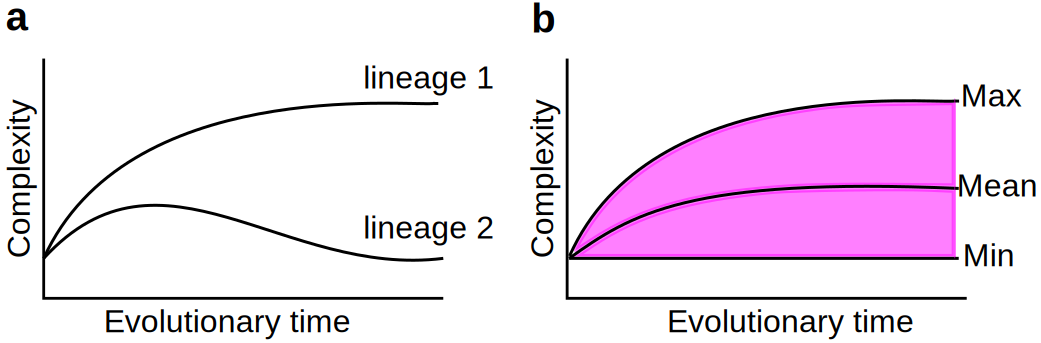
\includegraphics[width=12cm]{./Images/complexity_min.jpeg}
  \centering
  \caption{a) Two lineages with different complexity change through their evolutionary trajectories.
  b) Representation of the minimum, mean and maximum complexity of many lineages over evolutionary time in which the minimum stay constant while the mean and maximum increase.
Redrawn from \citep{Arthur2010}.
 }
  \label{fig:Complexity_min}
\end{figure}
%%%%%%%%%%%%%%%%%%%%%%%%%%%%%%%%%%%%%%%%%%%%%%%%%%%%%%%%%%%%%%%%%%%%%%%%%%%%%%%%%%%%%

\subsection{Complexity Increase in Development}

The increase in complexity in an organism during embryogenesis is probably one of the most intuitive processes of animal development.
It is commonly seen even as one of its defining characteristics.
Eric H. Davidson described the progressive increase in complexity as the "essence" of development \citep{Davidson2001}. Despite of the widely accepted view of complexity increase in development, there is no consensus of how to define it, much less on how to quantify it \citep{susan2000ontogeny}.

Using the number of cell types again as a proxy of morphological complexity, it can be said that during metazoan development, complexity increases as the zygote divides and differentiates into an adult with multiple cell types. 
This simple definition of complexity has its complications, as there is no clear criteria of how to define a cell type or how to determine when a new cell type has formed during development. 
For example, it could be that at the morphological level a cell seems to be undifferentiated, but when isolating it from its neighbour cells, it differentiates in an autonomous way into a specific cell type, suggesting that the cell fate was already determined without the necessity of further interactions with other cells.

\textbf{Talk about differentiation and determination?}

 
In addition, this definition does not take into account that embryos do not only get more cell types, but these cell types become organized in specific patterns in space and time in the embryo, which also could be considered as an increase in complexity over developmental time.

%%%%%%%%%%%%%%%%%%%%%%%%%%%%%%%%%%%%%%%%%%%%%%%%%%%%%%%%%%%%%%%%%%%%%%%%%%%%%%%%%%%%%
%\clearpage
\begin{mdframed}[style=boxstyle,frametitle={Box1. On the similarity of complexity patterns between Evolution and Development}]\label{Box1:Haeckel&vonBaer}

The connection between the increase in complexity during development and evolutionary time it has been largely discussed.
Haeckel was one of the first who made explicit hypothesis about the connection between the development and evolutionary patterns.
In what is known as Haeckel's "Biogenetic Law", he described development (or ontogeny), as a brief summary of the slow and long phylogeny \citep{haeckel1874menschen}.
In his hypothesis, a "higher" organism would pass through a series of conserved developmental stages that represent ancestral forms. This view is also known as the "recapitulation theory".

Karl Ernst von Baer, an Estonian naturalist, also formulated his own hypotheses, known as von Baer's laws \citep{vonBaer1828uber}. He stated that general characteristics develop before special characteristics (first law) and, opposed to Haeckel, that the embryo of a "higher" animal never resembles the adult of another animal form, but only his embryo (fourth law). 

Apart from the differences in the "recapitulation" view, Haeckel and von Baer \citep{Richardson2002} they disagreed in the acceptance of evolution. 
Haeckel's view was an evolutionary one, while von Baer's was not. Curiously, von Baer's arguments were used by Darwin in its "Origin" \citep{darwin1859origin} to support common ancestry and therefore, evolution.

Now is evident that any of these hypotheses can be considered "laws", as they are not universal. They only apply to some characters, stages and levels of phylogenetic inclusiveness \citep{Richardson2002}. Nevertheless, both Haeckel and von Baer work represented the foundations of the comparative embryology field, which is in turn the basis of the modern evolutionary developmental biology (evo-devo).
	\nomenclature{Evo-devo}{Evolutionary Developmental Biology}
\end{mdframed}
%%%%%%%%%%%%%%%%%%%%%%%%%%%%%%%%%%%%%%%%%%%%%%%%%%%%%%%%%%%%%%%%%%%%%%%%%%%%%%%%%%%%%

Defining a pattern as a specific distribution of cell types in a specific temporal window of embryonic development \citep{Salazar-Ciudad2004}, development can be conceptualized as the continuous transformation of one pattern into another.
The earliest pattern transformations usually establish the main axis or "compartments" of the embryo. For example, the anterior/posterior and dorsal/ventral axes in the fruit fly.
	\nomenclature{A/P}{anterior/posterior}
	\nomenclature{D/V}{dorsal/ventral}
Later pattern transformations define smaller compartments of the embryo, e.g, limbs, fingers  or internal organs.
As development proceeds, spatial compartments are progressively specified at an increasing finer resolution \citep{Davidson2001}.
Thus, a great part of pattern transformation is the partition of specific embryo compartments into smaller sub-compartments.

The compartmentalization of the embryo can be considered then an intrinsic property of development, and, as it is going to be mention in later sections, can be used as a proxy of complexity.

\subsection{Complexity at the molecular level}

At the molecular level, the increasing compartmentalization of the embryo during development can be seen as the progressive spatial restriction of gene expression to subsequently smaller regions in the embryo.
Sean Carroll conceptualizes this process\citep{Carroll2001} as:
%%%%%%%%%%%%%%%%%%%%%%%%%%%%%%%%%%%%%%%%%%%%%%%%%%%%%%%%%%%%%%%%%%%%%%%%%%%%%%%%%%%%
\begin{enumerate}
\item In early development, genes have a broad expression in the embryo and define the main axes of the body.
\item Later, genes define smaller compartments like organs and appendages (field-specific selector genes).
\item Finally, genes become expressed in specific cell types like muscle and neural cells (cell-type specific selector genes). 
\end{enumerate}
%%%%%%%%%%%%%%%%%%%%%%%%%%%%%%%%%%%%%%%%%%%%%%%%%%%%%%%%%%%%%%%%%%%%%%%%%%%%%%%%%%%%
%This would imply that in general, the area of expression of a gene in the embryo (relative to the area of the whole embryo)

If we consider again the number of cells as the complexity measure, we would expect that the increase in complexity over developmental time (as the number of cell types augments), should be associated with an underlying increase in complexity at the molecular level \citep{Arthur2010}, following the reasoning that:

%%%%%%%%%%%%%%%%%%%%%%%%%%%%%%%%%%%%%%%%%%%%%%%%%%%%%%%%%%%%%%%%%%%%%%%%%%%%%%%%%%%%
\begin{enumerate}
\item In development, the morphological complexity increases with time, as new cell types form.
\item Different cell-types are characterized by the differential expression of genes.
\item Therefore, the more cell-types an organism is formed of, more different combinations of expressed genes has to have (with the gene regulatory complexity this must entail).
\end{enumerate}
%%%%%%%%%%%%%%%%%%%%%%%%%%%%%%%%%%%%%%%%%%%%%%%%%%%%%%%%%%%%%%%%%%%%%%%%%%%%%%%%%%%%

The above reasoning has lead to some researchers to propose that the complexity of an organism resides in the regulatory machinery that ends into the differentiation of the diverse cell types \citep{Davidson2001}. 

For some, the combinatorial approach could also be seen as the solution for the "G-value paradox", as what really matters to be complex would not be how many genes an organism has, but how would these genes are differentially combined to produce more cell types in it.

The differential gene expression in the various number of cell types are determined in great manner by the interplay of genes and their \textit{cis}-regulatory regions (DNA regions usually close to a gene which contains specific sequence motifs where proteins bind and affect its expression). The interaction between genes and their \textit{cis}-regulatory regions is sometimes referred as gene regulatory networks (GRNs) or "regulatory architecture" of the genome \citep{Davidson2001}.
	\nomenclature{GRN}{Gene Regulatory Network}



\subsection{Complexity in informational terms}

\cite{Davidson2001} used above mentioned concepts in addition to others to explain development (and evolution) on informational terms. He said that development (which is the outcome of spatial and temporal series of differential gene expression) is controlled by a hardwired regulatory program built into the DNA and the metric of complexity is the diversity of the programs of gene expression that are "installed and executed" as the embryo develops. As Davidson, other authors have used informational/computational analogies to define development \citep{Apter1965,monod2012cytodifferentiation,mayr1997evolution} 

To illustrate how the complexity of a regulatory network or "program" can increase in evolution (but a similar case could be said for development), Davidson describes an imaginary example:
an early evolutionary state consists of a small gene battery (set of functionally linked genes expressed in concert) encoding proteins used for some differentiated cell type, which is activated by a small number of genes encoding transcription factors. The network activating the gene battery is itself controlled by a single upstream gene.
In subsequent evolutionary states, the whole structure is said to become more complex as: the battery of genes is now used in some pattern formation system, new batteries of genes appear, new regulatory genes and new \textit{cis}-regulatory regions are introduced  \citep{Davidson2001}.

Even when in this kind of examples would seem easy to discern a simple GRN from a complex one just from its topology, the high intricacy of real biological systems make this an extremely difficult if not impossible task. 
Additional levels of complexity have to be taken into account, like feedback effects and the non-linear regulation of gene expression, which make the prediction of changes in regulatory states hard or even impossible to predict \citep{Jaeger2014devmech}.

There are also important critiques of this informational approach. First, using an informational analogy to describe development implies the distinction between a "hardware" and a "software".
The "hardware" would consist of the genome structure, regulatory components, cells, organs, etc., and the "sofware" would be the GRNs or the set of instructions that directs the performance of specific operations.
For biological systems, this distinction is misleading, as there are recurrent feedback between its "hardware" and "software", so that the structure of development processes change through development \citep{susan2000ontogeny,Salazar-Ciudad2009,Jaeger2014devmech}.


\subsection{Complexity in terms of dynamical systems theory}

Estimating the combinatorial possibilities of a small set of regulatory genes, considering that each gene can regulate (whether positively or negatively) more than one gene's expression in addition to its own, could result in an astronomic number of possible gene topologies.



increased in complexity as:

- cis-regulatory regions GRN (davidson)

- miRNA

- nothing about spatial or statistical approach like our disparity measure


explain something about non-genetic components (Newman, Gabor and Forgacs, Alberch, Isaac)



%%%%%%%%%%%%%%%%%%%%%%%%%%%%%%%%%%%%%%%%%%%%%%%%%%%%%%%%%%%%%%%%%%%%%%%%%%%%%%%%%%%%%
\begin{figure}[h]
  \includegraphics[width=5cm]{./Images/GRNs.png}
  \centering
  \caption{
  Some GRNs
 }
  \label{fig:GRNs}
\end{figure}
%%%%%%%%%%%%%%%%%%%%%%%%%%%%%%%%%%%%%%%%%%%%%%%%%%%%%%%%%%%%%%%%%%%%%%%%%%%%%%%%%%%%%
